% Contents\
\begin{abstract}
    In this work, I explore the exercises on the final assignment of Signal
    Processing: Principles and Applications. The work centres around adaptive
    filter and the normalized least mean squares algorithm.
\end{abstract}

\section{Exercise 1}

In this exercise, and for each of the three signals in study, I decided to test
three different filter orders (\(n\)), with three different adaptation steps
(\(\mu\)). These are:
\begin{equation}
    \begin{aligned}
        n   & = {3, 5, 10}      \\
        \mu & = {0.3, 0.5, 0.9}
    \end{aligned}
\end{equation}

The experiment is done by script {\tt experiment1.m} and supported by the function
    {\tt do\_nlms.m}. Furthermore, plotting is handled by the Python script {\tt
        makeplots\_1.py}.

There is a lot to unpack here, so let's get started. The first signal a sequence
of random numbers that is filtered and to which is added some white noise
component. The filter is given by:
\begin{equation}
    F(Z) = \frac{Z+2Z^{-1}}{Z+0.5Z^{-1}}
\end{equation}
This filter has one pole and one zero. Figure~\ref{fig:ex1varystep} shows how the
adaptation evolves in regarding to the adaptation step. Keep in mind that, as
asked, the adaptation step goes down by a factor of 10 in the middle of the
adaptation.
\begin{figure}
    \centering
    \begin{subfigure}[t]{0.32\columnwidth}
        \centering
        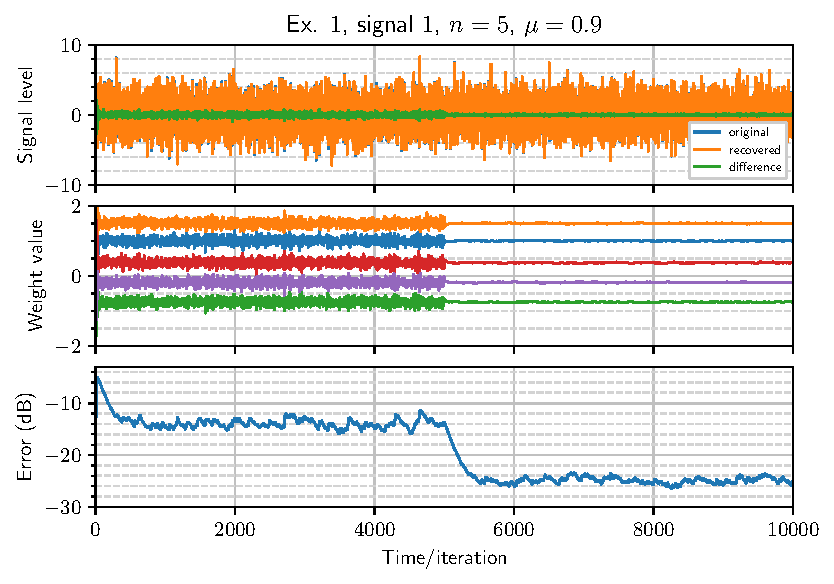
\includegraphics[width=\columnwidth]{pdf/ex1_l1_n5_mu90.pdf}
        \caption{}
    \end{subfigure} \hfill
    \begin{subfigure}[t]{0.32\columnwidth}
        \centering
        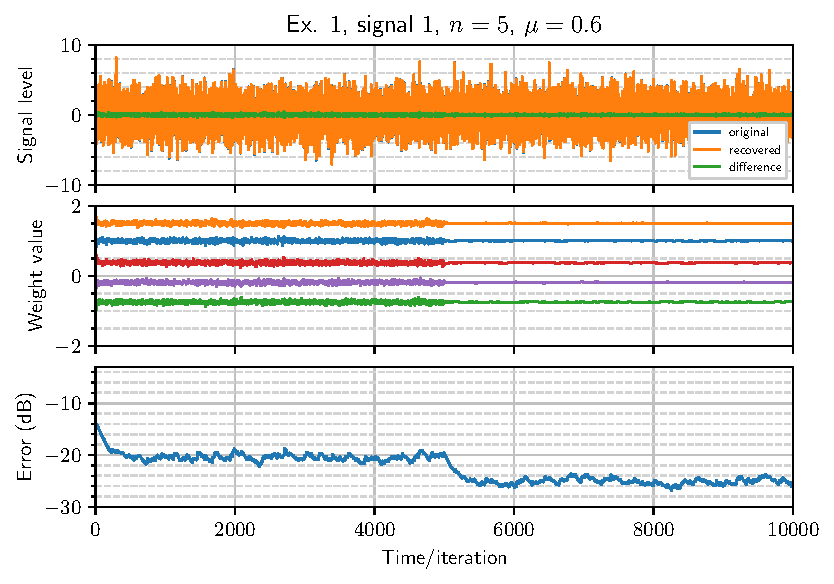
\includegraphics[width=\columnwidth]{pdf/ex1_l1_n5_mu60.pdf}
        \caption{}
    \end{subfigure} \hfill
    \begin{subfigure}[t]{0.32\columnwidth}
        \centering
        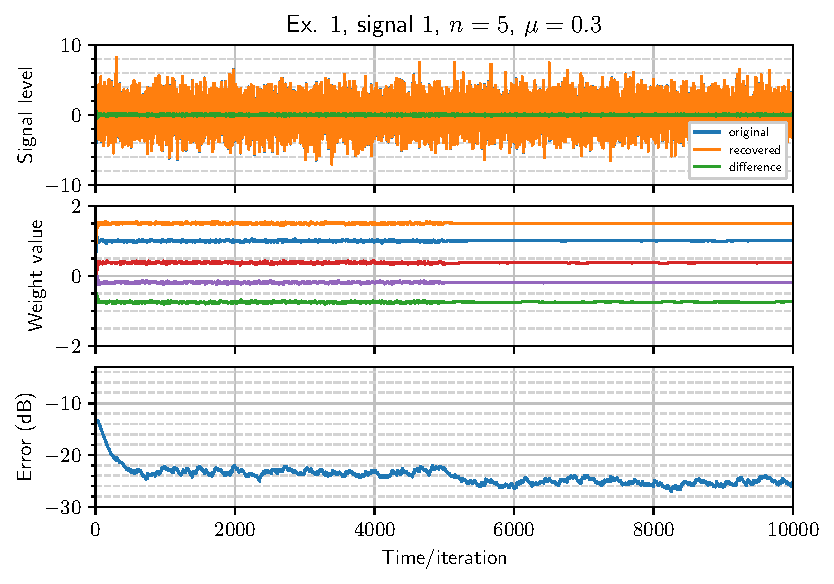
\includegraphics[width=\columnwidth]{pdf/ex1_l1_n5_mu30.pdf}
        \caption{}
    \end{subfigure}
    \caption{Results for the first signal of exercise 1: varying adaptation
        step.\label{fig:ex1varystep}}
\end{figure}
We see nothing too extraordinary: with smaller adaptation steps, the error is
smaller. This is the intuitive results, however, one must note that this might not
always be the case: a slow adaptation step can cause problems on dynamic systems,
as the adaptive filter might not adapt fast enough. Also, with smaller adaptation
steps, the level of error (which is equivalent to a noise floor of the system) is
not only lower but less jittery. We can think of this optimization problem as
looking for solutions in a convex space: smaller adaptation steps correspond to a
smaller oscillation in the bottom of the concave surface. We see that with a
filter order of 3 the noise floor is between \SI{-24}{\decibel} to
\SI{-26}{\decibel}. Of course that the next step is to compare this floor in
regard to the filter order. Figure~\ref{fig:ex1varyorder} shows this.
\begin{figure}
    \centering
    \begin{subfigure}[t]{0.32\columnwidth}
        \centering
        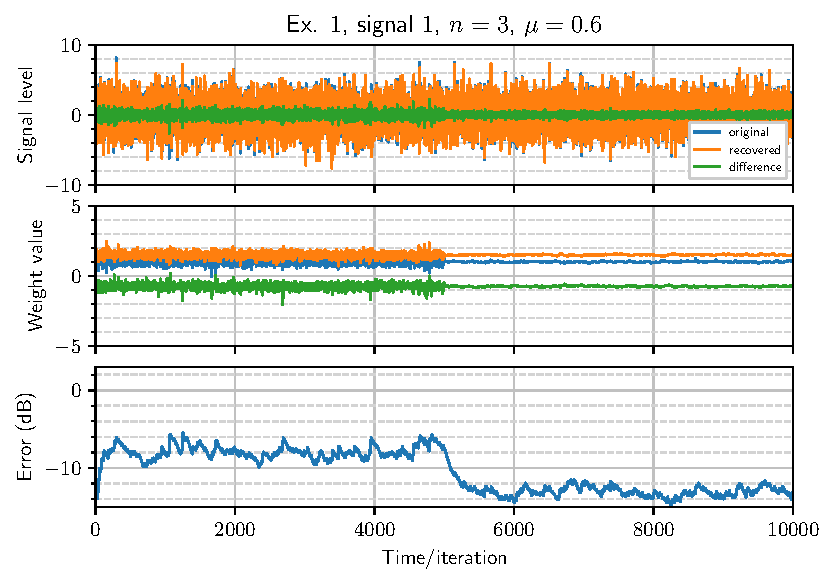
\includegraphics[width=\columnwidth]{pdf/ex1_l1_n3_mu60.pdf}
        \caption{}
    \end{subfigure} \hfill
    \begin{subfigure}[t]{0.32\columnwidth}
        \centering
        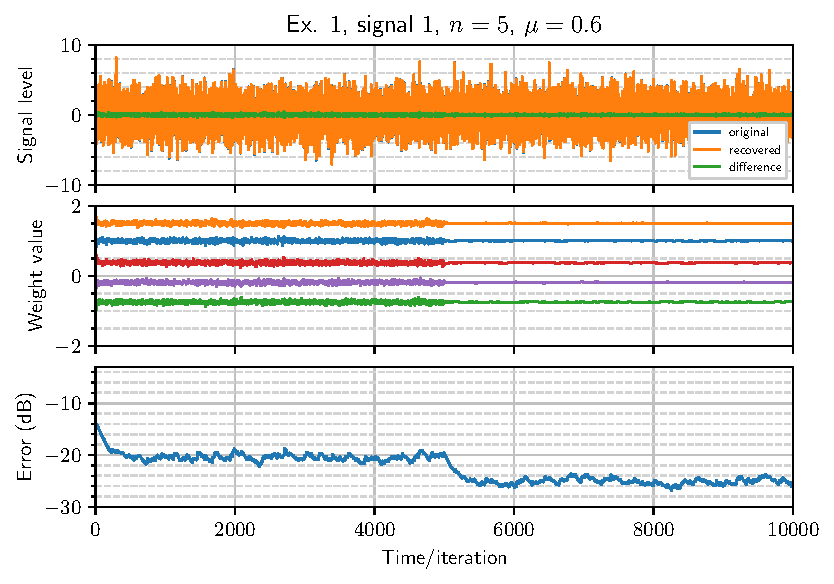
\includegraphics[width=\columnwidth]{pdf/ex1_l1_n5_mu60.pdf}
        \caption{}
    \end{subfigure} \hfill
    \begin{subfigure}[t]{0.32\columnwidth}
        \centering
        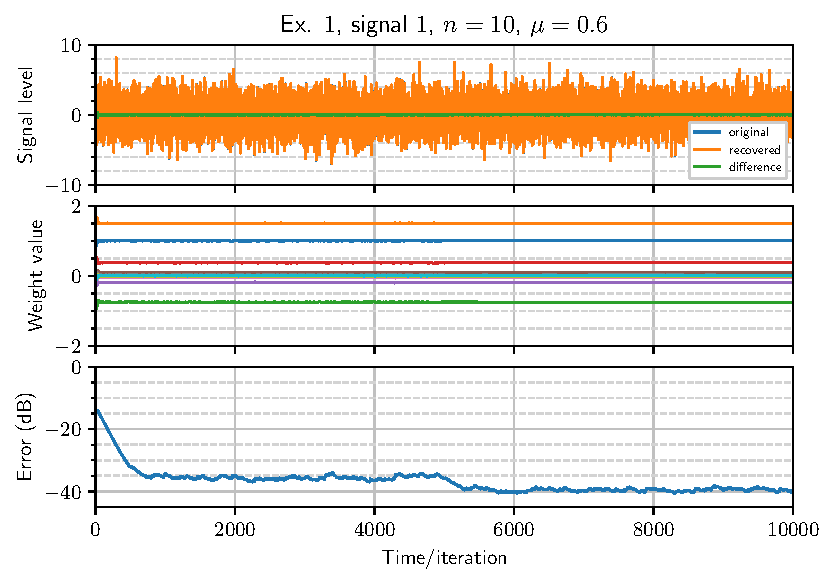
\includegraphics[width=\columnwidth]{pdf/ex1_l1_n10_mu60.pdf}
        \caption{}
    \end{subfigure}
    \caption{Results for the first signal of exercise 1: varying filter
        order.\label{fig:ex1varyorder}}
\end{figure}
We see that for the same adaptation step, increasing the filter order decreases
both the error of the adaptation and the fluctuations of the weights of the
filter.

With the second signal, things get more interesting. In
figure~\ref{fig:ex1sig2switch}, we can see an interesting effect: in the first
sinusoidal section, the weight marked in blue has a larger value than the one in
orange, situation that inverts in the second case. Since a sinusoidal is fully
described by amplitude and phase, the system is overdetermined. The converge to
specific set of weights is not deterministic. We observe the adaptation step is
the most relevant factor in the sinusoidal regions and that the number of weights
becomes more important in the other regions.
\begin{figure}
    \centering
    \begin{subfigure}[t]{0.32\columnwidth}
        \centering
        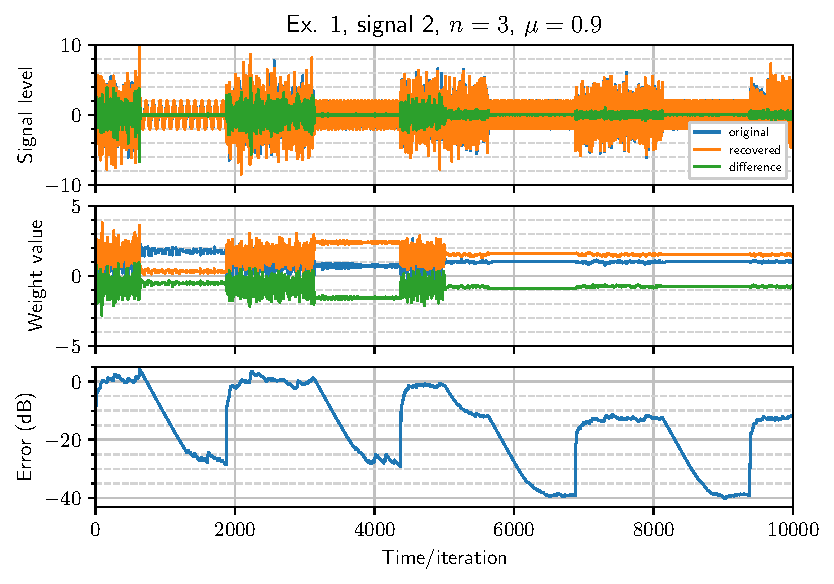
\includegraphics[width=\columnwidth]{pdf/ex1_l2_n3_mu90.pdf}
        \caption{\label{fig:ex1sig2switch}}
    \end{subfigure} % \hspace{1cm}
    \begin{subfigure}[t]{0.32\columnwidth}
        \centering
        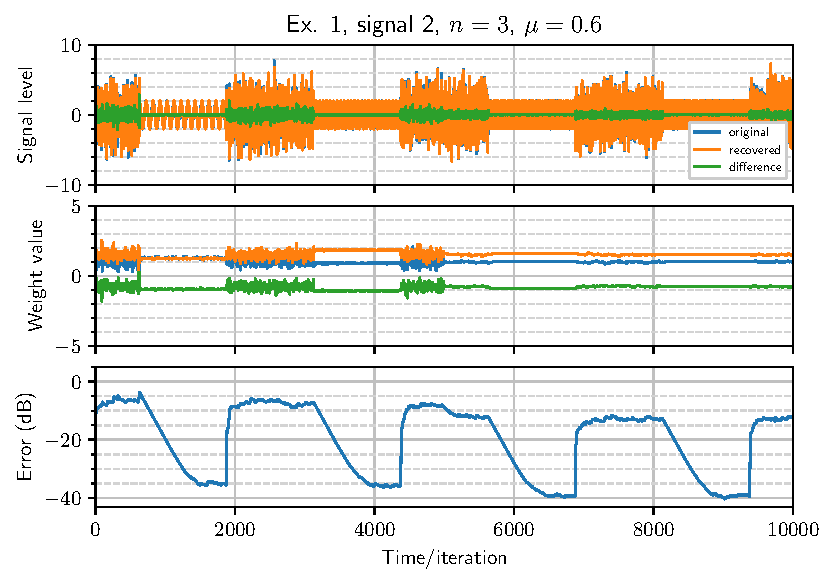
\includegraphics[width=\columnwidth]{pdf/ex1_l2_n3_mu60.pdf}
        \caption{}
    \end{subfigure} \\
    \begin{subfigure}[t]{0.32\columnwidth}
        \centering
        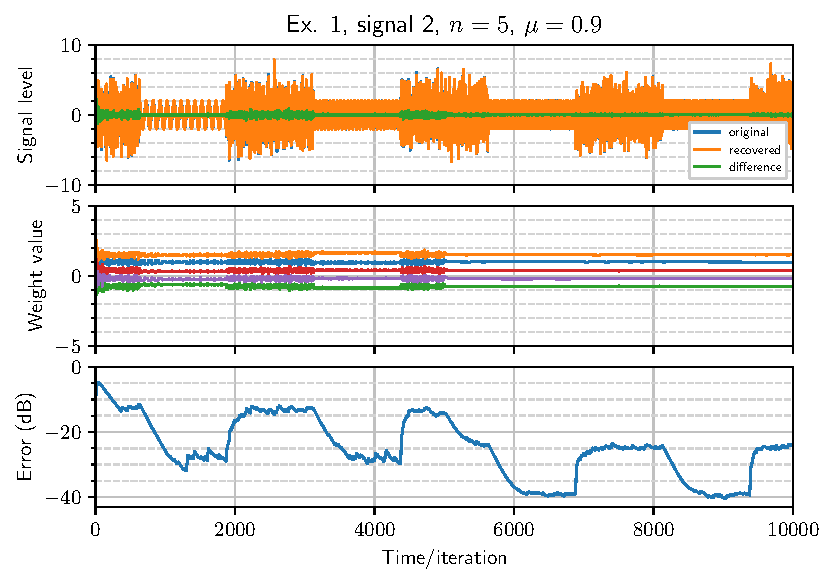
\includegraphics[width=\columnwidth]{pdf/ex1_l2_n5_mu90.pdf}
        \caption{}
    \end{subfigure} % \hspace{1cm}
    \begin{subfigure}[t]{0.32\columnwidth}
        \centering
        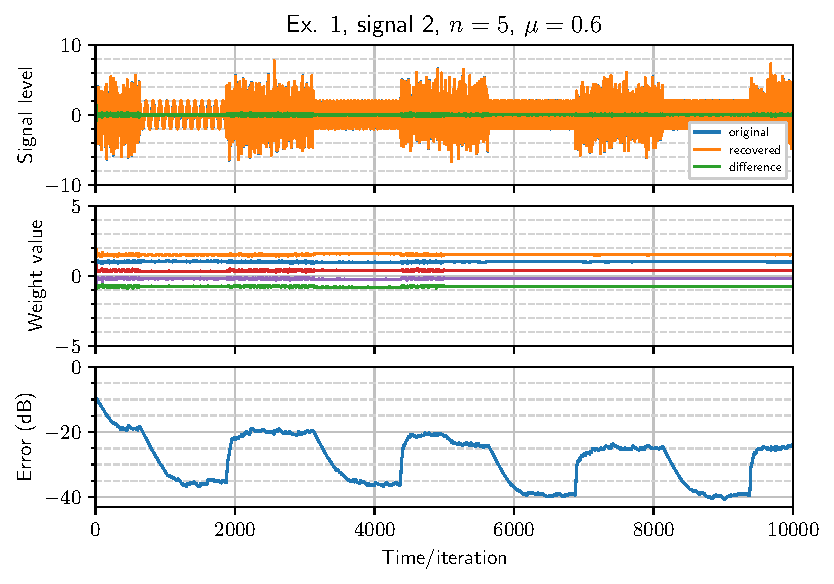
\includegraphics[width=\columnwidth]{pdf/ex1_l2_n5_mu60.pdf}
        \caption{}
    \end{subfigure}
    \caption{Results for the second signal of exercise 1.\label{fig:ex1sig2}}
\end{figure}

The last signal is probably the most interesting one to analyse.
Figure~\ref{fig:ex1vsig3} depicts the results for this exercise.
\begin{figure}[t!]
    \centering
    \begin{subfigure}[t]{0.32\columnwidth}
        \centering
        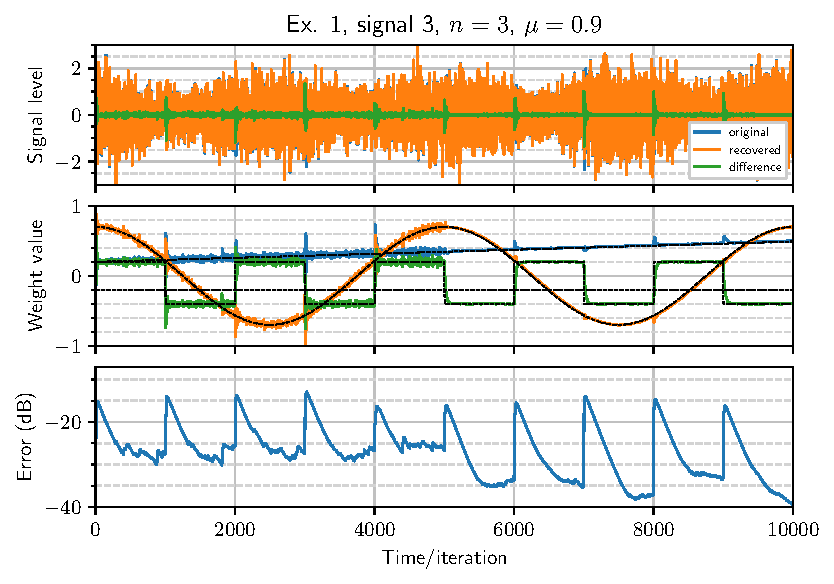
\includegraphics[width=\columnwidth]{pdf/ex1_l3_n3_mu90.pdf}
        \caption{}
    \end{subfigure} \hfill
    \begin{subfigure}[t]{0.32\columnwidth}
        \centering
        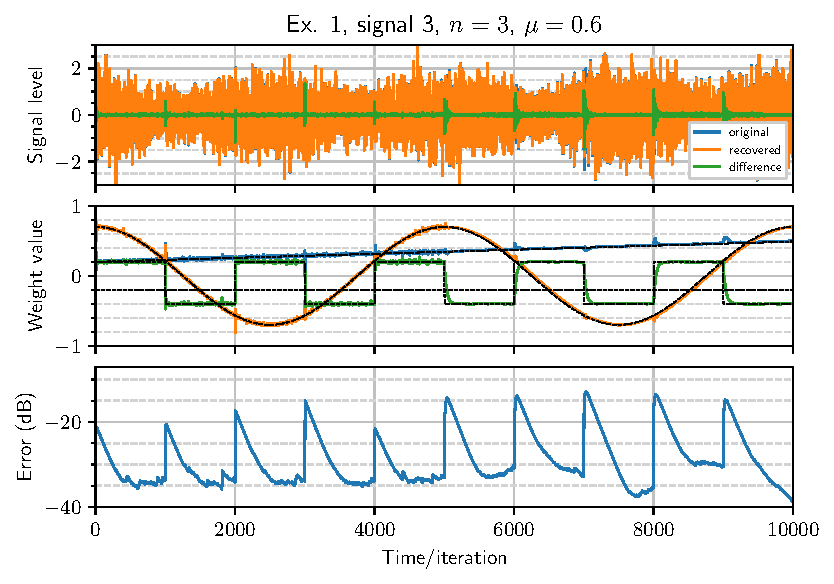
\includegraphics[width=\columnwidth]{pdf/ex1_l3_n3_mu60.pdf}
        \caption{}
    \end{subfigure} \hfill
    \begin{subfigure}[t]{0.32\columnwidth}
        \centering
        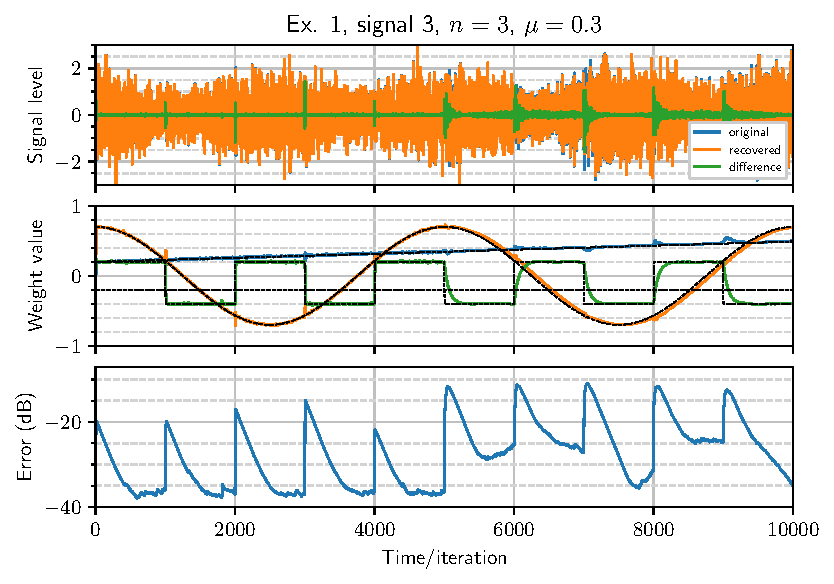
\includegraphics[width=\columnwidth]{pdf/ex1_l3_n3_mu30.pdf}
        \caption{}
    \end{subfigure} \\
    \begin{subfigure}[t]{0.32\columnwidth}
        \centering
        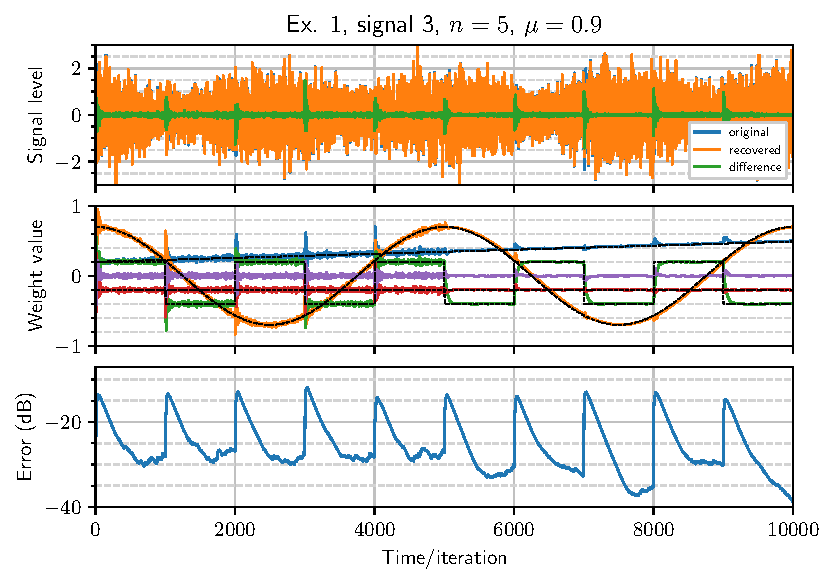
\includegraphics[width=\columnwidth]{pdf/ex1_l3_n5_mu90.pdf}
        \caption{}
    \end{subfigure} \hfill
    \begin{subfigure}[t]{0.32\columnwidth}
        \centering
        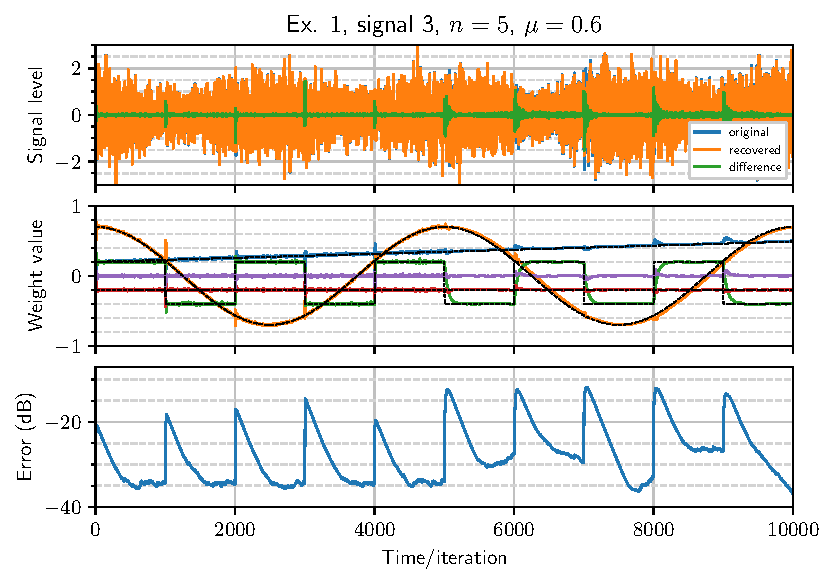
\includegraphics[width=\columnwidth]{pdf/ex1_l3_n5_mu60.pdf}
        \caption{}
    \end{subfigure} \hfill
    \begin{subfigure}[t]{0.32\columnwidth}
        \centering
        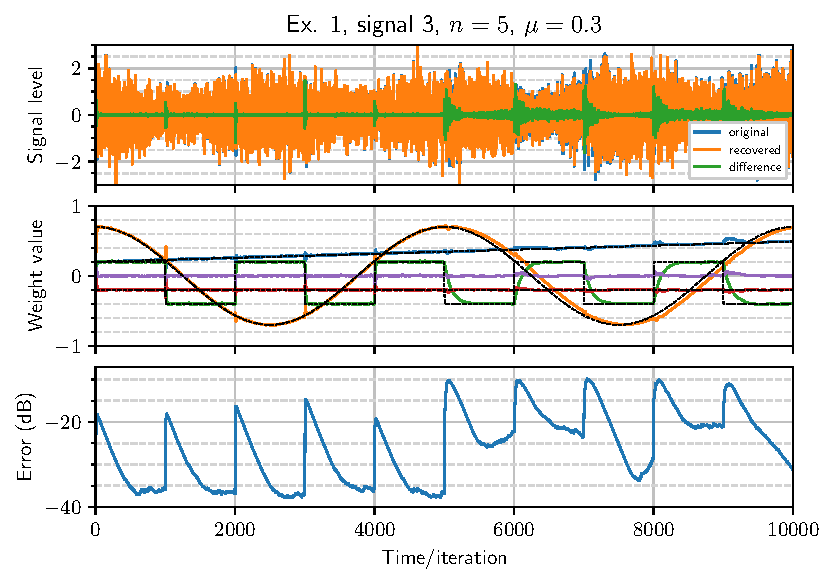
\includegraphics[width=\columnwidth]{pdf/ex1_l3_n5_mu30.pdf}
        \caption{}
    \end{subfigure} \\
    \begin{subfigure}[t]{0.32\columnwidth}
        \centering
        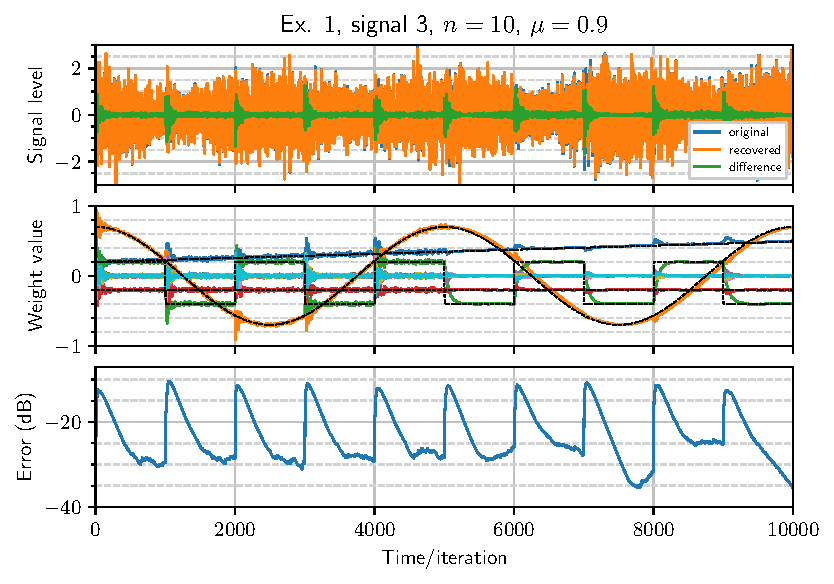
\includegraphics[width=\columnwidth]{pdf/ex1_l3_n10_mu90.pdf}
        \caption{}
    \end{subfigure} \hfill
    \begin{subfigure}[t]{0.32\columnwidth}
        \centering
        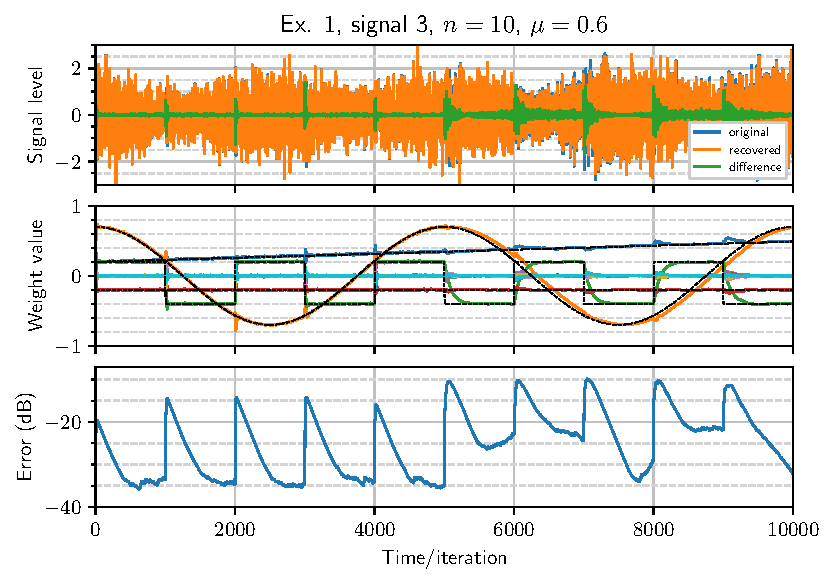
\includegraphics[width=\columnwidth]{pdf/ex1_l3_n10_mu60.pdf}
        \caption{}
    \end{subfigure} \hfill
    \begin{subfigure}[t]{0.32\columnwidth}
        \centering
        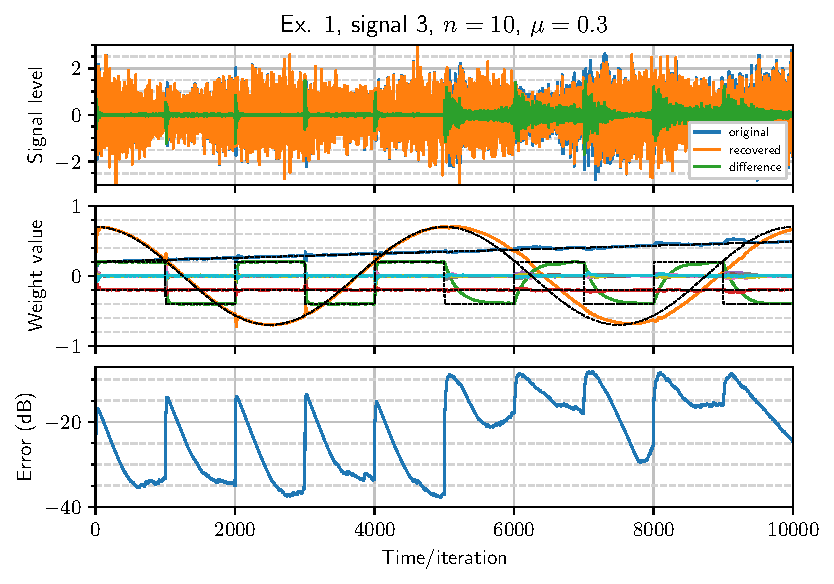
\includegraphics[width=\columnwidth]{pdf/ex1_l3_n10_mu30.pdf}
        \caption{\label{fig:ex1vsig3n10mu3}}
    \end{subfigure}
    \caption{Results for the third signal of exercise. The black dashed lines on
        the second subplot in each figure corresponds to the theoretical weights.
        \label{fig:ex1vsig3}}
\end{figure}
The way the figures are displayed, vertically we can see the effect of changing
the number of weights and horizontally the effect of improving the adaptation
step. We can see that for the coarser adaptation step, there is a lot of jittering
in the weights every time there is an abrupt change in the weights. In a way, we
can say the weights lost ``synchronization'' with the system and it needs to
recover. The behaviour is similar to a weakly damped oscillation after an impulse
impulse, hinting about the stability of the algorithm. On the other hand, on the
finer adaptation steps, two effects become clearly visible. One is that the
adaptation clearly starts to lag behind the ideal weights. The second, especially
visible in the weight that varies as a square wave, is that there is a clear
low-pass filter effect. This can get really extreme. I'd like to point out the
particular case of the figure~\label{fig:ex1vsig3n10mu3} for \(n=10\) and
\(\mu=0.3\) where we can see that in the first part the error is actually lower
than in the second part, where \(\mu=0.03\). The effect of an adaptation that is
too slow becomes clearly visible with the decrease in performance.

\section{Exercise 2}

In exercise 2, we are to consider three signals:
\begin{align}
    x_1 (t) & = v(t) + 3v(t-1) + 3v(t-2)  \\
    x_2 (t) & = 3v(t) + 3v(t-1) + 1v(t-2) \\
    d(t)    & = v(t) - 2v(t-1) + v(t-2)
\end{align}
where \(v(t)\) is a Gaussian white noise stochastic process with zero mean and
unit variance.

In the first part of the exercise, we are asked to compute the autocorrelation of
each \(x_i\) signal and the cross-correlation between \(x_i\) and \(d\) for each
\(i\). I will present the process for one of them, since the other ones are
analogous. I'll do the autocorrelation of \(x_1\), denoted \(r_{x_1x_1}(k)\):
\begin{equation}
    r_{x_1x_1}(k) = \left< x_1 (t+k), x_1(t) \right>
\end{equation}
The first step is to expand \(x_1\):
\begin{equation}
    r_{x_1x_1}(k) = \left< v(t+k) + 3v(t-1+k) + 3v(t-2+k),
    v(t) + 3v(t-1) + 3v(t-2) \right>
\end{equation}
The inner product operation has the distributive property, so this is equivalent
to:
\begin{equation}
    \begin{aligned}
        r_{x_1x_1}(k) & = \left< v(t+k), v(t) \right>        \\
                      & + \left< v(t+k), 3v(t-1) \right>     \\
                      & + \left< v(t+k),  3v(t-2) \right>    \\
                      & + \left< 3v(t-1+k), v(t) \right>     \\
                      & + \left< 3v(t-1+k), 3v(t-1) \right>  \\
                      & +\left< 3v(t-1+k),  3v(t-2) \right>  \\
                      & + \left< 3v(t-2+k), v(t) \right>     \\
                      & + \left< 3v(t-2+k), 3v(t-1) \right>  \\
                      & + \left< 3v(t-2+k),  3v(t-2) \right> \\
    \end{aligned}
\end{equation}
Now we should pay close attention to this expression. Since \(v(t)\) is a Gaussian
stochastic process:
\begin{equation}
    \left<v(t-k),v(t-n)\right>=\begin{cases}
        1 & \text{if~} k=n   \\
        0 & \text{otherwise}
    \end{cases}
\end{equation}
Which massively simplifies the problem. For example, for \(k=-1\), only the second
and sixth parcels contribute to the result. And on these, it's just a matter of
multiplying the weights of the parcels together and then sum them.

We are also asked to confirm the results with simulation data. For that, I created
the MATLAB script {\tt experiment21.m}. It uses MATLAB's filter function to apply
the \(k\)-th delay to the signal. Since it's not possible to do such filter for
positive \(k\), what I do is delay the other signal instead.
Table~\ref{tab:results21} shows both the analytical and simulated results, as well
as the relative error for the simulated data.

\begin{table}[b!] \adjustbox{width=\columnwidth,keepaspectratio}{
        \begin{tabular}{|c|c|c|c|c|c|c|c|c|c|c|c|c|c|c|c|c|c|c|c|c|}
    \hline
    \multirow{3}{*}{\(k\)} & \multicolumn{5}{c|}{\(r_{x_1x_1}\)} & \multicolumn{5}{c|}{\(r_{x_1d}\)} & \multicolumn{5}{c|}{\(r_{x_2x_2}\)} & \multicolumn{5}{c|}{\(r_{x_2d}\)}\tabularnewline
    \cline{2-21} \cline{3-21} \cline{4-21} \cline{5-21} \cline{6-21} \cline{7-21} \cline{8-21} \cline{9-21} \cline{10-21} \cline{11-21} \cline{12-21} \cline{13-21} \cline{14-21} \cline{15-21} \cline{16-21} \cline{17-21} \cline{18-21} \cline{19-21} \cline{20-21} \cline{21-21}
     & \multirow{2}{*}{Analyt.} & \multicolumn{4}{c|}{Sim.} & \multirow{2}{*}{Analyt.} & \multicolumn{4}{c|}{Sim.} & \multirow{2}{*}{Analyt.} & \multicolumn{4}{c|}{Sim.} & \multirow{2}{*}{Analyt.} & \multicolumn{4}{c|}{Sim.}\tabularnewline
    \cline{3-6} \cline{4-6} \cline{5-6} \cline{6-6} \cline{8-11} \cline{9-11} \cline{10-11} \cline{11-11} \cline{13-16} \cline{14-16} \cline{15-16} \cline{16-16} \cline{18-21} \cline{19-21} \cline{20-21} \cline{21-21}
     &  & \(n=n_1\) & rel.\ error (\%) & \(n=n_2\) & rel.\ error (\%) &  & \(n=n_1\) & rel.\ error (\%) & \(n=n_2\) & rel.\ error (\%) &  & \(n=n_1\) & rel.\ error (\%) & \(n=n_2\) & rel.\ error (\%) &  & \(n=n_1\) & rel.\ error (\%) & \(n=n_2\) & rel.\ error (\%)\tabularnewline
    \hline
    \(-3\) & \(0\) & \(0.00740\) &  & \(-0.00138\) &  & \(0\) & \(0.01074\) &  & \(0.00051\) &  & \(0\) & \(0.01948\) &  & \(-0.00004\) &  & \(0\) & \(-0.00062\) &  & \(0.00000\) & \tabularnewline
    \hline
    \(-2\) & \(3\) & \(3.04359\) & \(14.53\) & \(3.00077\) & \(0.05\) & \(1\) & \(1.00635\) & \(6.35\) & \(0.99961\) & \(0.06\) & \(3\) & \(3.01627\) & \(5.42\) & \(3.00004\) & \(0.01\) & \(3\) & \(3.00270\) & \(0.90\) & \(2.99994\) & \(0.06\)\tabularnewline
    \hline
    \(-1\) & \(12\) & \(12.05903\) & \(4.92\) & \(12.00114\) & \(0.23\) & \(1\) & \(0.98318\) & \(16.82\) & \(0.99962\) & \(0.02\) & \(12\) & \(12.01831\) & \(1.53\) & \(12.00006\) & \(0.04\) & \(-3\) & \(-3.00103\) & \(-0.34\) & \(-2.99988\) & \(-0.36\)\tabularnewline
    \hline
    \(0\) & \(19\) & \(19.04664\) & \(2.45\) & \(19.00069\) & \(0.28\) & \(-2\) & \(-1.99454\) & \(-2.73\) & \(-1.99976\) & \(-0.09\) & \(19\) & \(19.02250\) & \(1.18\) & \(19.00009\) & \(0.07\) & \(-2\) & \(-2.00287\) & \(-1.44\) & \(-2.00021\) & \(-0.15\)\tabularnewline
    \hline
    \(1\) & \(12\) & \(12.05903\) & \(4.92\) & \(12.00114\) & \(0.23\) & \(-3\) & \(-2.99158\) & \(-2.81\) & \(-2.99982\) & \(-0.06\) & \(12\) & \(12.01831\) & \(1.53\) & \(12.00006\) & \(0.04\) & \(1\) & \(1.00332\) & \(3.32\) & \(1.00021\) & \(0.06\)\tabularnewline
    \hline
    \(2\) & \(3\) & \(3.04359\) & \(14.53\) & \(3.00077\) & \(0.05\) & \(3\) & \(2.98048\) & \(6.51\) & \(2.99947\) & \(0.08\) & \(3\) & \(3.01627\) & \(5.42\) & \(3.00004\) & \(0.01\) & \(1\) & \(1.00081\) & \(0.81\) & \(1.00000\) & \(0.00\)\tabularnewline
    \hline
    \(3\) & \(0\) & \(0.00740\) &  & \(-0.00138\) &  & \(0\) & \(0.00979\) &  & \(-0.00013\) &  & \(0\) & \(0.01948\) &  & \(-0.00004\) &  & \(0\) & \(-0.00716\) &  & \(-0.00068\) & \tabularnewline
    \hline
    \end{tabular}

    } \caption{Results for the first part of exercise 2. \(n_1=1000000\) and
        \(n_2=ns = 100000000\)\label{tab:results21}}
\end{table}

The second part of the exercise asks us to solve the system of normal equations
for various number of weights and to plot the error as function of this. Results
for this can be seen in figures~\ref{fig:ex22x1} and~\ref{fig:ex22x2}.
\begin{figure}
    \centering
    \begin{minipage}[t]{0.32\columnwidth}
        \centering
        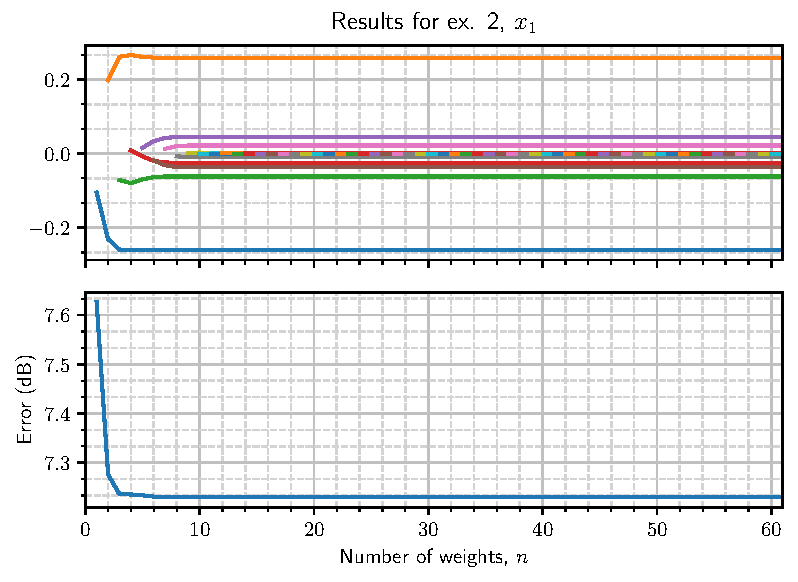
\includegraphics[width=\columnwidth]{pdf/ex2_pt2_x1_all.pdf}
        \caption{Results for the second part of ex. 2 for \(x_1(t)\)
            \label{fig:ex22x1}}
    \end{minipage}
    \hspace{1cm}
    \begin{minipage}[t]{0.32\columnwidth}
        \centering
        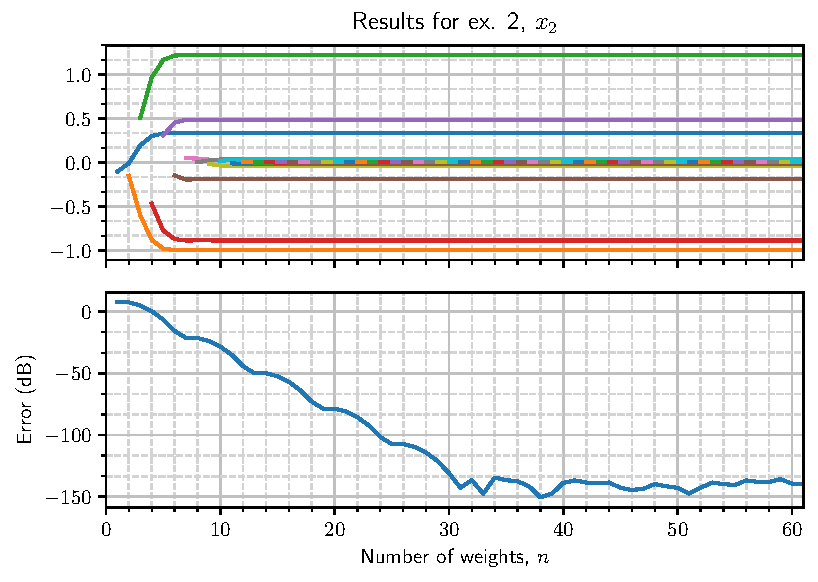
\includegraphics[width=\columnwidth]{pdf/ex2_pt2_x2_all.pdf}
        \caption{Results for the second part of ex. 2 for \(x_2(t)\)
            \label{fig:ex22x2}}
    \end{minipage}
\end{figure}
We see immediately that for the \(x_1\) the error never leaves the
\SI{7}{\decibel} range, regardless of the filter order. On the other hand, for
\(x_2\) we see a clear convergence to around \SI{-150}{\decibel}, coherent with
limitations of floating point arithmetic.
% To understand why, let's look at the characteristics of \(x_1\) and \(x_2\). We
% can say \(x_1(t)\) is obtained from \(v(t)\) by a filter of the form \(Z +
% 3Z^{-1} + 3Z^{-2}\) and \(x_2(t)\) from a filter of the form \(3Z + 3Z^{-1} +
% Z^{-2}\). The first one has roots outside the unit circle while the roots of the
% later one are inside the unit circle. Having the zeros outside the unit circle
% means one of two things: if we choose as the region of convergence (ROC) the
% inner circle, we have a system that is stable, but is anti-causal. On the other
% hand, if we choose as the ROC the external region of the Z-plane the system
% becomes causal, but at the cost of stability.

\FloatBarrier
\section{Exercise 3}

In exercise 3, we are asked to use the NMLS algorithm to make an adaptive filter
that works with the previous signals. For this, I sidestepped a bit from script.
The number of iterations and the step were both too low to see the best converge
possible. The same with the number of weights. I settled on two million iterations
and \(40\) weights. For the iteration step I did something else: the script adapts
the weights as iterations go along, as can be seen in line 47 of {\tt
experiment3.m}. Results can be seen in figure~\ref{fig:ex3res}. For the case of
\(x_1\) we see an agreement with the analytical prediction, with an error floating
around \SI{7}{\decibel}. The error jitters around this value, and it's interesting
to see how little the error does vary with the clear jittering of the weight
themselves. This gives strength to the hypothesis that the system has a very
non-causal response and that this causal filter cannot actually do much to
compensate. For \(x_2\) we see quite the opposite. Visually, one can't even see
variation in the weights after the initial adjustment and still the error keeps
dropping down until almost half-way. It's interesting to see that the noise floor
is around \SI{-170}{\decibel}, \SI{20}{\decibel} lower than even the analytical
predictions. Finally, let's compare the final values of the filter coefficients in
both cases, again the previous exercise. For the sake of simplicity, I show the 10
most important weights for each case. The results can be seen in
table~\ref{tab:results2}. I purposely let the large number of significant digits
in the case for \(x_2\) as it transmits the message of how similar these are. For
\(x_1\) results are less equal, which is easy to understand given the large jitter
of these results.
\begin{figure}[h!]
    \centering
    \begin{subfigure}[t]{0.32\columnwidth}
        \centering
        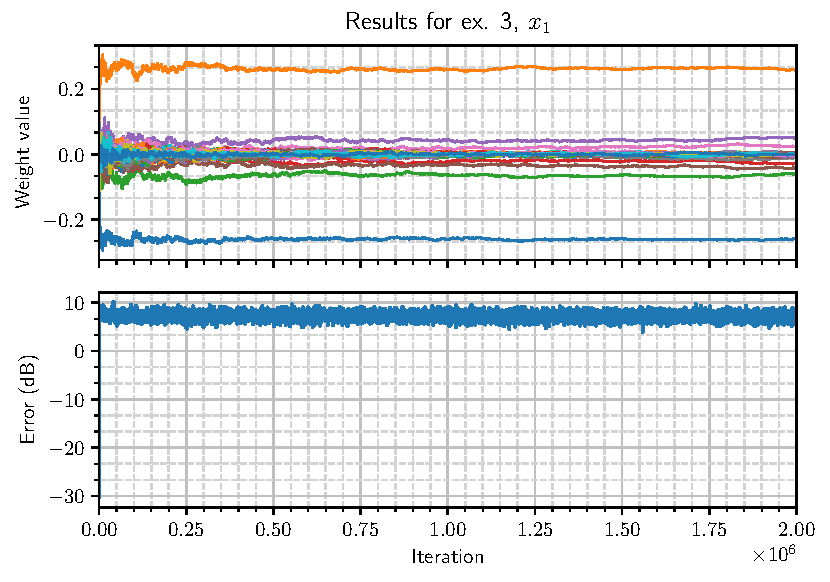
\includegraphics[width=\columnwidth]{pdf/ex3_x1_all.pdf}
        \caption{Results for \(x_1\).}
    \end{subfigure} \hspace{1cm}
    \begin{subfigure}[t]{0.32\columnwidth}
        \centering
        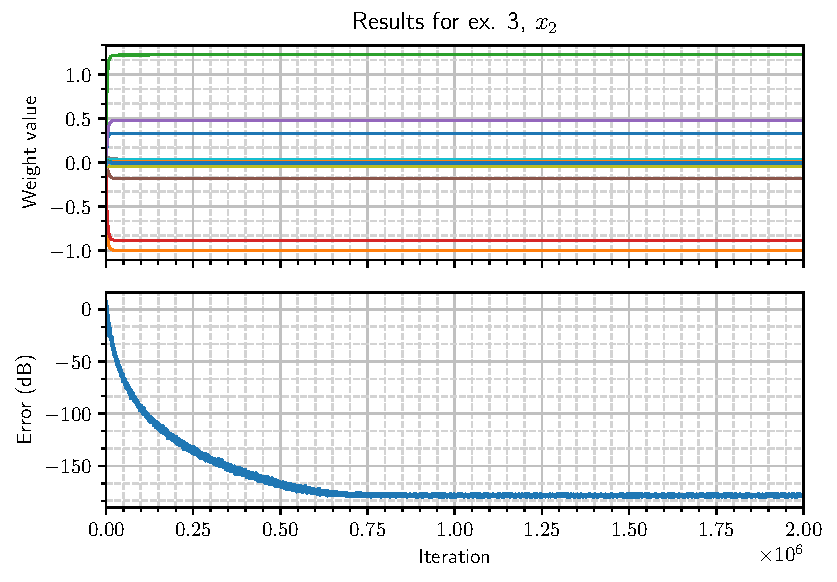
\includegraphics[width=\columnwidth]{pdf/ex3_x2_all.pdf}
        \caption{Results for \(x_2\).}
    \end{subfigure}
    \caption{Results for the exercise 3.\label{fig:ex3res}}
\end{figure}
\begin{table}[h!]
    \centering
    \scalebox{0.65}{
        \begin{tabular}{|c|c|c|c|}
    \hline
    \multicolumn{2}{|c|}{\(x_{1}\)} & \multicolumn{2}{c|}{\(x_{2}\)}\tabularnewline
    \hline
    \hline
    Analytical & Simulation & Analytical & Simulation\tabularnewline
    \hline
    \(0.25926\) & \(0.25943\) & \(1.222222222222\) & \(1.222222222225\)\tabularnewline
    \hline
    \(-0.25926\) & \(-0.25791\) & \(-1.000000000000\) & \(-1.000000000002\)\tabularnewline
    \hline
    \(-0.06173\) & \(-0.06163\) & \(-0.888888888889\) & \(-0.888888888892\)\tabularnewline
    \hline
    \(0.04527\) & \(0.04390\) & \(0.481481481481\) & \(0.481481481483\)\tabularnewline
    \hline
    \(-0.03704\) & \(-0.03381\) & \(0.333333333333\) & \(0.333333333335\)\tabularnewline
    \hline
    \(-0.02469\) & \(-0.02547\) & \(-0.185185185185\) & \(-0.185185185187\)\tabularnewline
    \hline
    \(0.02195\) & \(0.01877\) & \(-0.045267489712\) & \(-0.045267489712\)\tabularnewline
    \hline
    \(-0.00960\) & \(-0.00739\) & \(0.037037037037\) & \(0.037037037037\)\tabularnewline
    \hline
    \(-0.00168\) & \(-0.00450\) & \(0.032921810700\) & \(0.032921810702\)\tabularnewline
    \hline
    \(-0.00081\) & \(-0.00434\) & \(0.024691358025\) & \(0.024691358025\)\tabularnewline
    \hline
\end{tabular}

    }
    \caption{Results for the exercise 3.\label{tab:results2}}
\end{table}

\FloatBarrier
\section{Exercise 4}

In exercise 4, we are asked to create an adaptive filter whose input is:
\begin{equation}
    x(t)=\cos(\omega t) + \sigma v(t)
\end{equation}
And the target signals are:
\begin{align}
    d_1 (t) & = x(t+1)                                                \\
    d_2 (t) & = =A(t)\sin(\omega t),\;A(t)=\begin{cases}
        +2 & t<5000          \\
        -2 & t\geqslant 5000
    \end{cases}
\end{align}
with \(\omega = 0.2\pi\) and \(\sigma = 0.01\). As per the assignment, I ran the
tests for \(n=\{1,\ 2,\ 3\}\) and \(\mu=\{0.1,\ 0.8\}\). Results can be seen in
figures~\ref{fig:ex4d1} and~\ref{fig:ex4d2}.
\begin{figure}[h!]
    \centering
    \begin{subfigure}[t]{0.32\columnwidth}
        \centering
        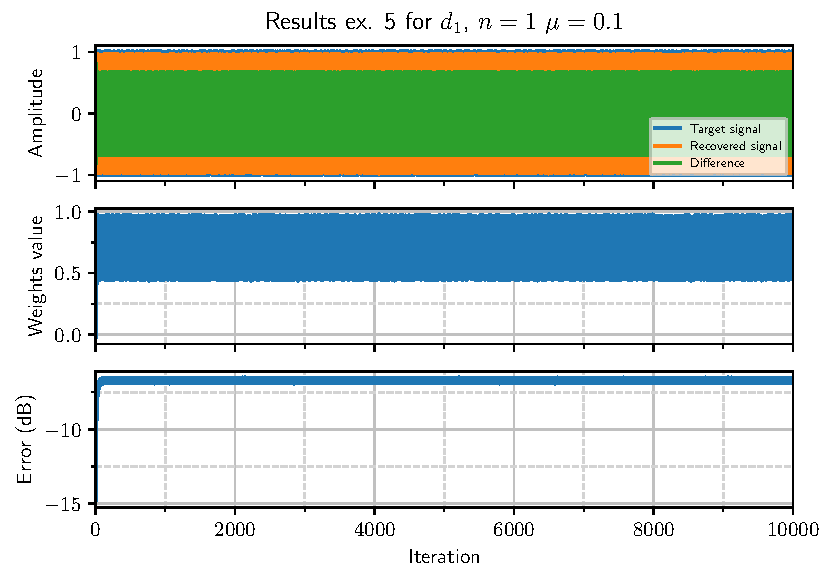
\includegraphics[width=\columnwidth]{pdf/results_ex4_d1_n1_mu0.10.pdf}
        \caption{}
    \end{subfigure} \hfill
    \begin{subfigure}[t]{0.32\columnwidth}
        \centering
        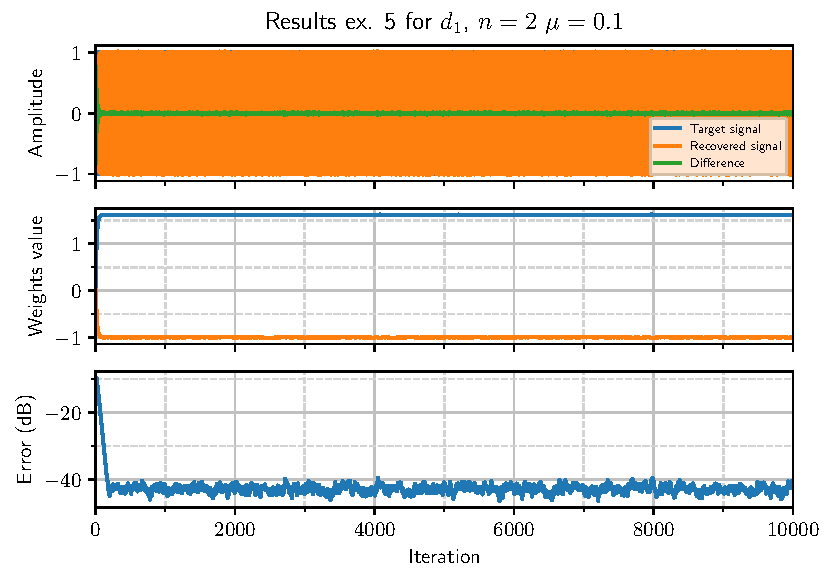
\includegraphics[width=\columnwidth]{pdf/results_ex4_d1_n2_mu0.10.pdf}
        \caption{}
    \end{subfigure} \hfill
    \begin{subfigure}[t]{0.32\columnwidth}
        \centering
        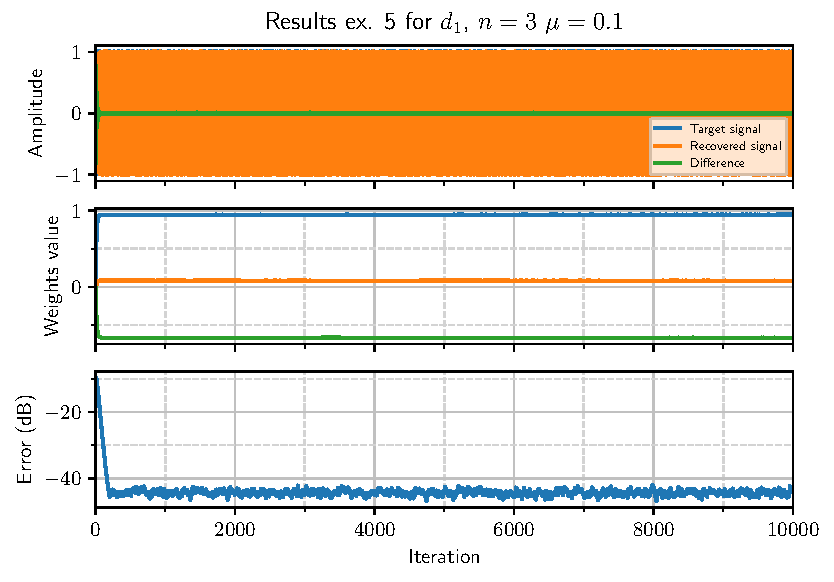
\includegraphics[width=\columnwidth]{pdf/results_ex4_d1_n3_mu0.10.pdf}
        \caption{}
    \end{subfigure} \\
    \begin{subfigure}[t]{0.32\columnwidth}
        \centering
        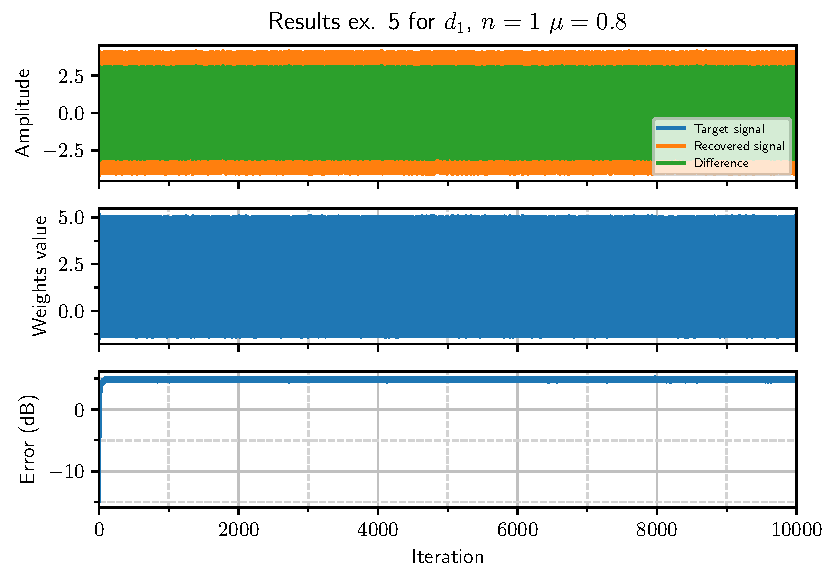
\includegraphics[width=\columnwidth]{pdf/results_ex4_d1_n1_mu0.80.pdf}
        \caption{}
    \end{subfigure} \hfill
    \begin{subfigure}[t]{0.32\columnwidth}
        \centering
        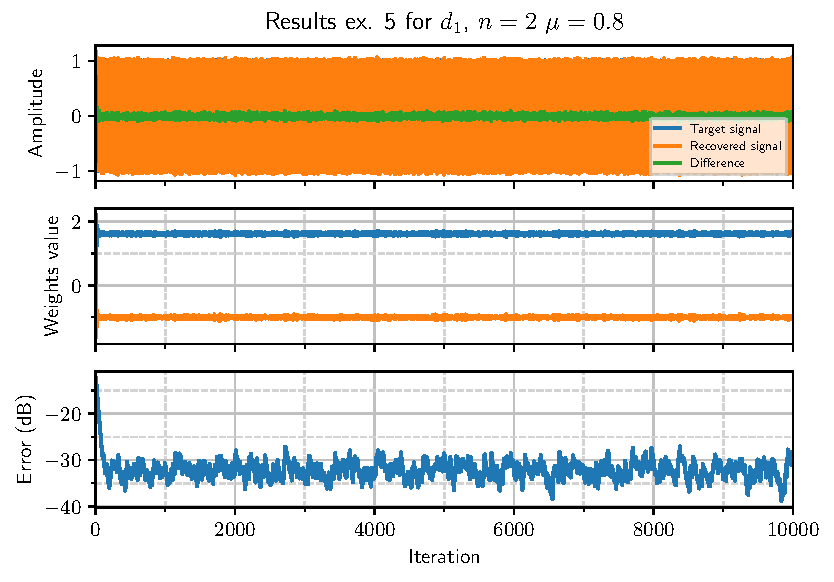
\includegraphics[width=\columnwidth]{pdf/results_ex4_d1_n2_mu0.80.pdf}
        \caption{}
    \end{subfigure} \hfill
    \begin{subfigure}[t]{0.32\columnwidth}
        \centering
        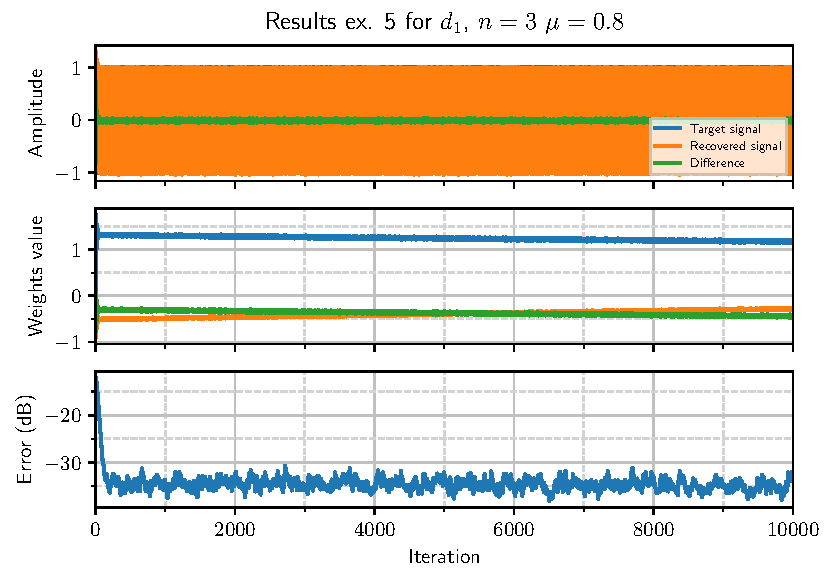
\includegraphics[width=\columnwidth]{pdf/results_ex4_d1_n3_mu0.80.pdf}
        \caption{\label{fig:ex4d1n3mu08}}
    \end{subfigure}
    \caption{Results for exercise 4, for \(d_1\).\label{fig:ex4d1}}
\end{figure}
\begin{figure}[h!]
    \centering
    \begin{subfigure}[t]{0.32\columnwidth}
        \centering
        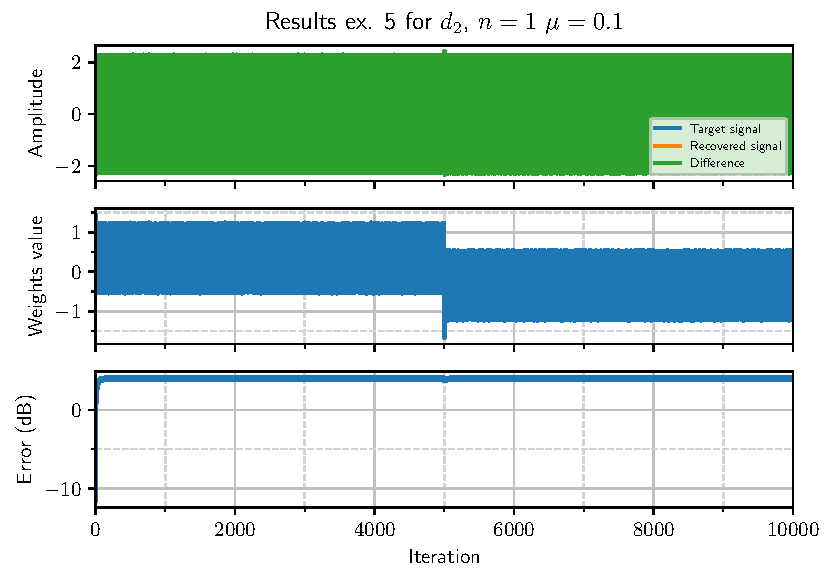
\includegraphics[width=\columnwidth]{pdf/results_ex4_d2_n1_mu0.10.pdf}
        \caption{}
    \end{subfigure} \hfill
    \begin{subfigure}[t]{0.32\columnwidth}
        \centering
        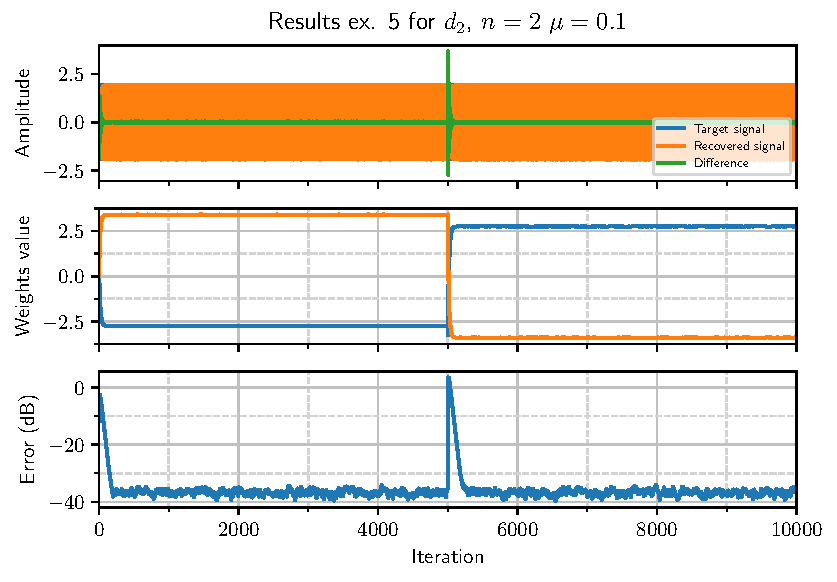
\includegraphics[width=\columnwidth]{pdf/results_ex4_d2_n2_mu0.10.pdf}
        \caption{}
    \end{subfigure} \hfill
    \begin{subfigure}[t]{0.32\columnwidth}
        \centering
        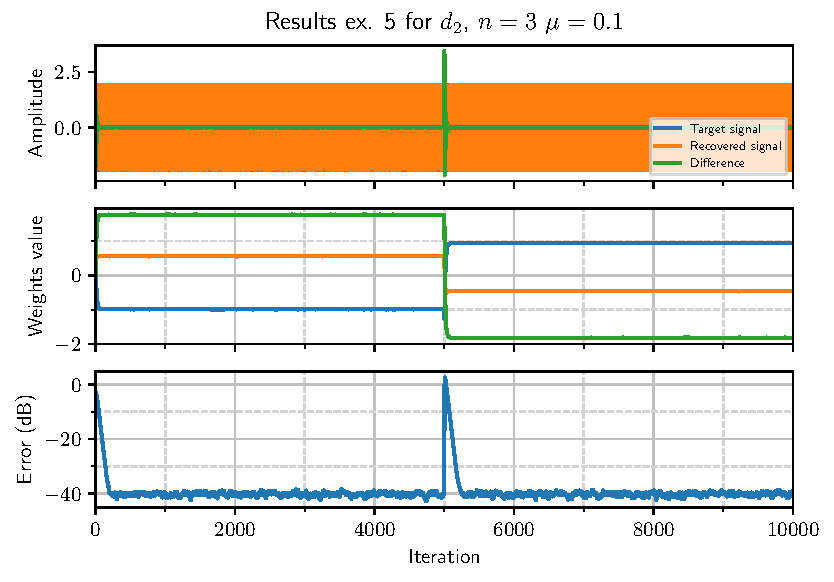
\includegraphics[width=\columnwidth]{pdf/results_ex4_d2_n3_mu0.10.pdf}
        \caption{}
    \end{subfigure} \\
    \begin{subfigure}[t]{0.32\columnwidth}
        \centering
        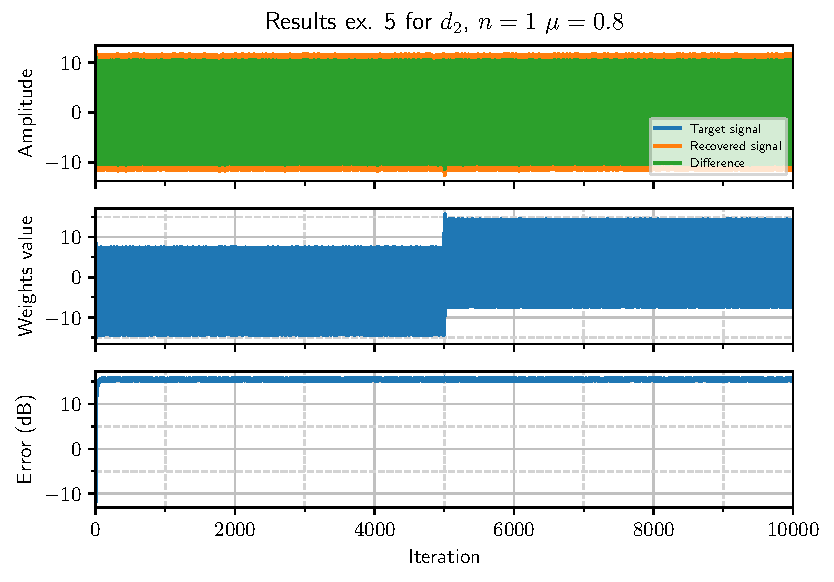
\includegraphics[width=\columnwidth]{pdf/results_ex4_d2_n1_mu0.80.pdf}
        \caption{}
    \end{subfigure} \hfill
    \begin{subfigure}[t]{0.32\columnwidth}
        \centering
        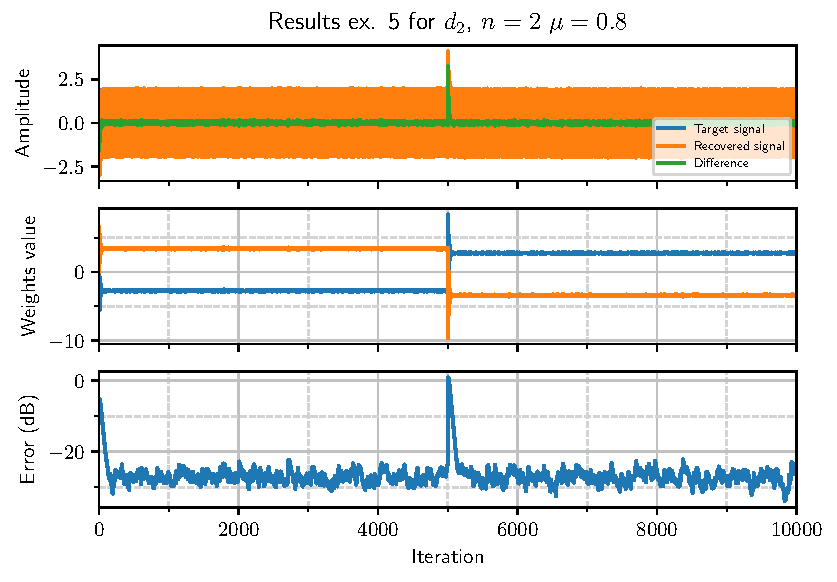
\includegraphics[width=\columnwidth]{pdf/results_ex4_d2_n2_mu0.80.pdf}
        \caption{}
    \end{subfigure} \hfill
    \begin{subfigure}[t]{0.32\columnwidth}
        \centering
        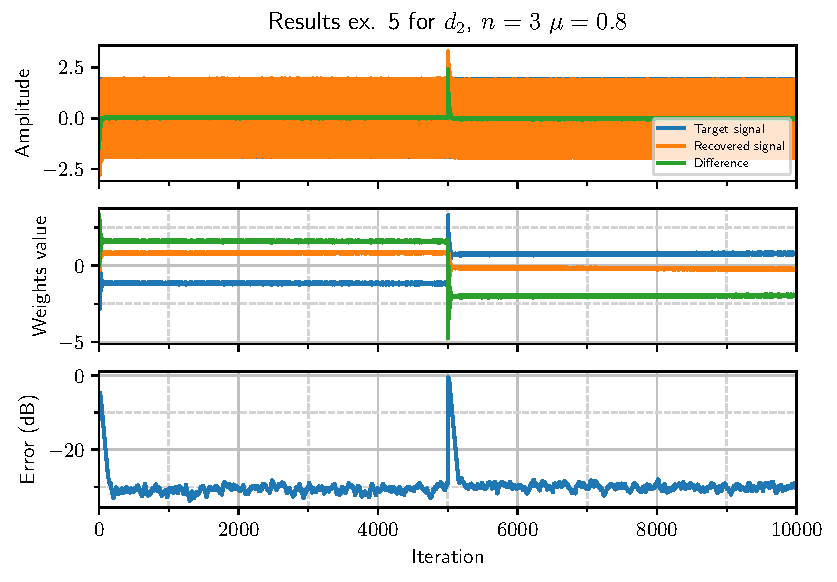
\includegraphics[width=\columnwidth]{pdf/results_ex4_d2_n3_mu0.80.pdf}
        \caption{\label{fig:ex4d2n3mu08}}
    \end{subfigure}
    \caption{Results for exercise 4, for \(d_2\).\label{fig:ex4d2}}
\end{figure}

Now let's look at these results. For either scenario, only one weight is not
enough. Between two and three weight there is barely any difference, even though
for \(n=3\) is slightly better. The filter is indeed able to predict the future
sample. As it was with the third signal on exercise 1, when \(d_2\) reverses the
amplitude we see the weights loose ``synchronization'' and then quickly pick up
again on the signals. I also want to point out the figure~\ref{fig:ex4d1n3mu08}
where we can see that the error barely changes but the weights keep evolving. This
might come from the system to be overdetermined. Also, on
figure~\ref{fig:ex4d2n3mu08} we can see that the adaptation on the second part is
slightly worse than from the first half. Even on the amplitude plot one can see
that the filter overcompensates and there is a slight DC shift on the recovered
signal, that stays below the original signal. I think that in this scenario
\(\mu\) is to high that any variation of the weights would make the adaptation
even worse, so this is why they don't change. Basically, the system would never be
able to fall into a better solution.This shows the importance of taking care into
using an appropriate adaptation step, and maybe even making this adaptation step
dynamic, for example, reducing it when the system reaches a steady state, so a
better solution can be searched for.

\FloatBarrier
\section{Exercise 5}

In exercise 5 we have a new challenge: we don't have a ``target'' signal. This
presents a very realistic scenario: if we had the target signal, what would be the
point of having an adaptive filter anyway? The challenge proposed to to make a
decision-directed adaptive filter for PSK signals. This means that to compute the
error we use the distance to the point in the PSK constellation we decided on
during demodulation. With this scheme, the received signal should tend to a good
PSK constellation. It's worth noting that without any further corrections, the
rotation of the constellation is not guaranteed to be correct.
Figure~\ref{fig:ex5_4psk} show the results for 4-PSK modulation using \(n=40\) and
\(\mu=0.1\) and figure~\ref{fig:ex5_8psk} show the results for 8-PSK modulation
using \(n=10\) and \(\mu=0.1\). It's interesting to see in
figures~\ref{fig:ex5_4psk_const} and~\ref{fig:ex5_8psk_const} how the
constellation does tend to the ``perfect'' one as the algorithm iterates. This is
an interesting way to visualize what the error evolution says.
\begin{figure}[h!]
    \centering
    \begin{subfigure}[t]{0.32\columnwidth}
        \centering
        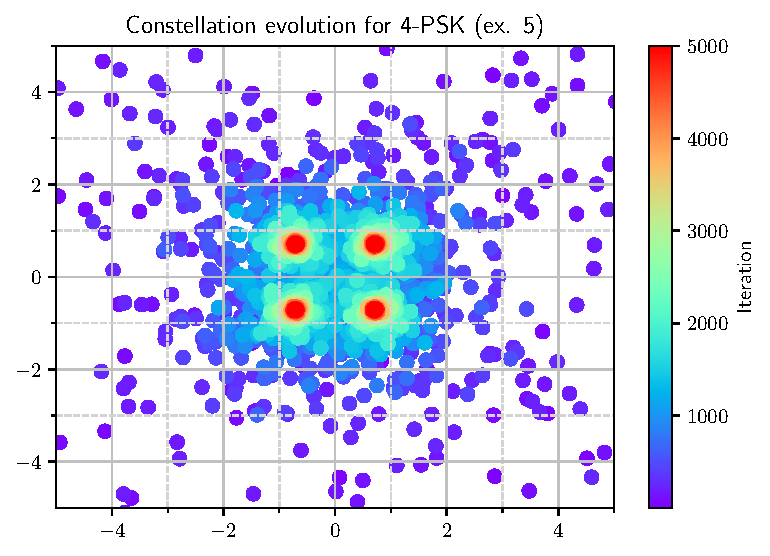
\includegraphics[width=\columnwidth]{pdf/ex5_4psk_const.pdf}
        \caption{Constellation evolution.\label{fig:ex5_4psk_const}}
    \end{subfigure} \hspace{1cm}
    \begin{subfigure}[t]{0.32\columnwidth}
        \centering
        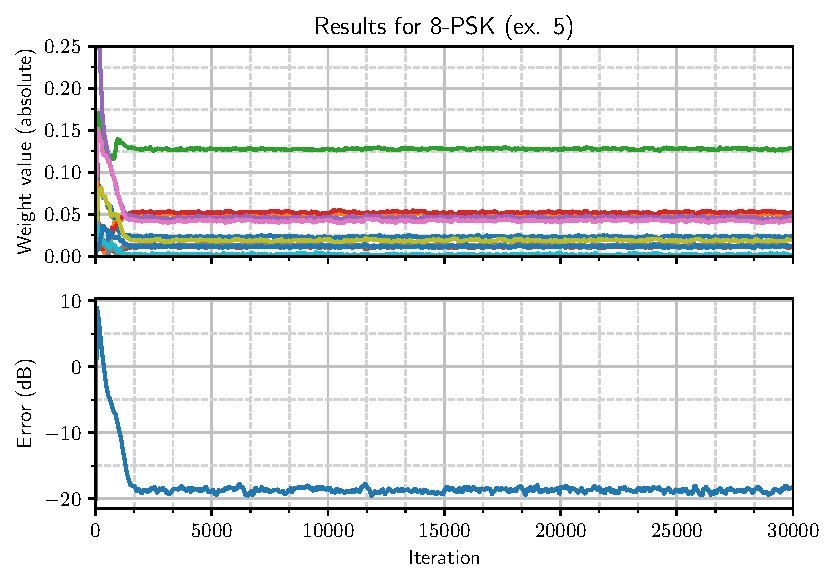
\includegraphics[width=\columnwidth]{pdf/ex5_8psk_res.pdf}
        \caption{Weights and error evolution.\label{fig:ex5_4psk_res}}
    \end{subfigure}
    \caption{Results for 4-PSK on exercise 5.\label{fig:ex5_4psk}}
\end{figure}
\begin{figure}[h!]
    \centering
    \begin{subfigure}[t]{0.32\columnwidth}
        \centering
        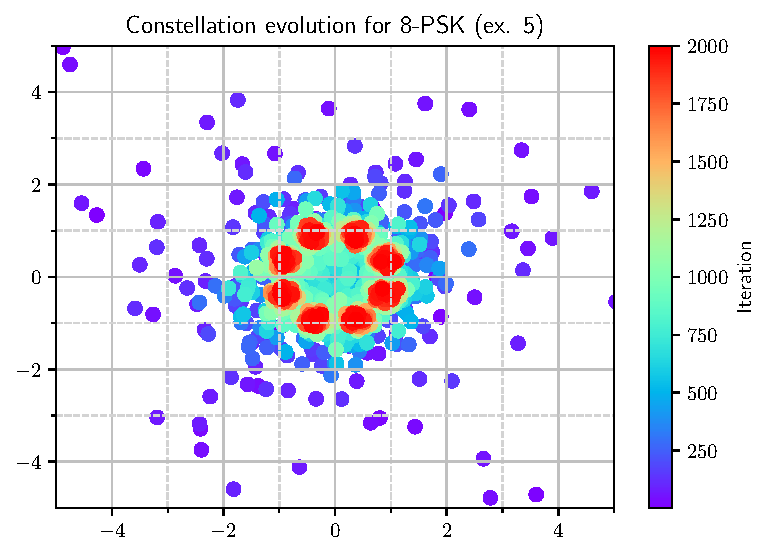
\includegraphics[width=\columnwidth]{pdf/ex5_8psk_const.pdf}
        \caption{Constellation evolution.\label{fig:ex5_8psk_const}}
    \end{subfigure} \hspace{1cm}
    \begin{subfigure}[t]{0.32\columnwidth}
        \centering
        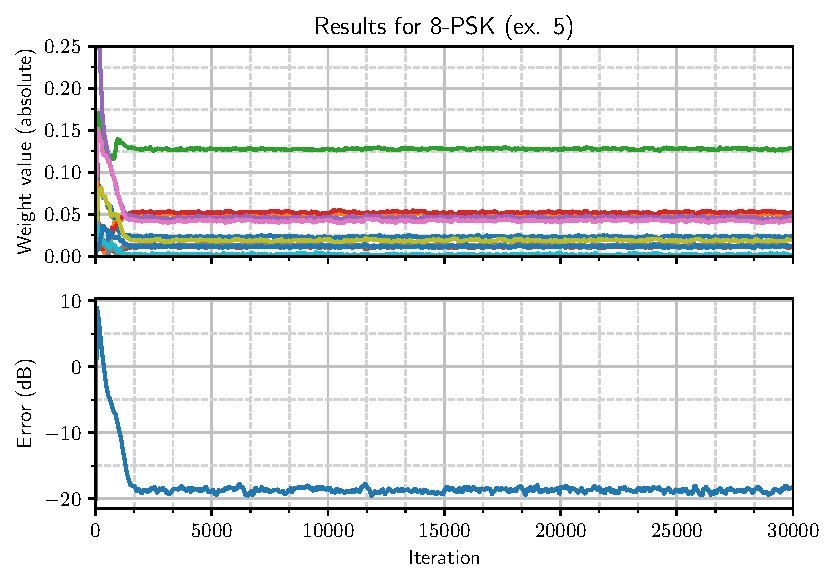
\includegraphics[width=\columnwidth]{pdf/ex5_8psk_res.pdf}
        \caption{Weights and error evolution.\label{fig:ex5_8psk_res}}
    \end{subfigure}
    \caption{Results for 8-PSK on exercise 5.\label{fig:ex5_8psk}}
\end{figure}
